\chapter{Results and Discussion} \label{chap:Results_and_Discussion}

\begin{table}[!hbt]
    \centering
    \caption[Explained Variance by different PCA settings]{\textbf{Explained Variance by different PCA settings.}.}
    \label{tab:PCA_Dimension}
    \pgfplotstabletypeset[
        every head row/.style={
            before row={
                \toprule
            },
            after row={
                \midrule
            },
        },
        every last row/.style={
            after row={
                \bottomrule
            },
        },
        begin table=\begin{tabular*}{.5\textwidth},
        end table=\end{tabular*},
        columns={0,1},
        columns/0/.style={int detect, multicolumn names=l,column name=\textbf{\#Components}, column type=@{\extracolsep{\fill}\hspace{6pt}}r},
        columns/1/.style={multicolumn names=l,column name=\textbf{Explained Variance}, column type=r}
    ]
    {Graphics/PCA.csv}
\end{table}

\begin{figure}
    \centering
    %\begin{adjustbox}{minipage=\dimexpr\textwidth-2\fboxsep-2\fboxrule,fbox}
    \begin{subfigure}[b]{0.475\textwidth}
        \caption[Dimension Reduction with \Acrshort{PCA}]{\textbf{Dimension Reduction with \Acrshort{PCA}}}
        \label{subfig:Normalisation_PCA}            \includegraphics[width=\textwidth]{PCA/Difference_Distance_Calculation.pdf}
    \end{subfigure}
    \hfill
    \begin{subfigure}[b]{0.475\textwidth}
        \caption[Dimension Reduction with \Acrshort{UMAP}]{\textbf{Dimension Reduction with \Acrshort{UMAP}}}
        \label{subfig:Normalisation_UMAP}            \includegraphics[width=\textwidth]{UMAP/Difference_Distance_Calculation.pdf}
    \end{subfigure}
    %\end{adjustbox}
    \caption[Cosine Distance Approximation with L2 Normalisation]{\textbf{Cosine Distance Approximation with L2 Normalisation.} .}
    \label{fig:Normalisation_Methods}
\end{figure}

\begin{figure}[!hbt]
    \centering
    %\includegraphics[width=\dimexpr\textwidth-2\fboxsep-2\fboxrule,fbox]{PCA/Data_Overview_Segment_4_H.pdf}
    \includegraphics[width=\textwidth]{PCA/Data_Overview_Segment_4_H.pdf}
    \caption[Segment 4 \Acrlong{HA} Antigen Subtype Frequency]{\textbf{Segment 4 \Acrlong{HA} Antigen Subtype Frequency.} .}
    \label{fig:Frequency_4}
\end{figure}

\begin{figure}[!hbt]
    \centering
    %\includegraphics[width=\dimexpr\textwidth-2\fboxsep-2\fboxrule,fbox]{PCA/Data_Overview_Segment_6_N.pdf}
    \includegraphics[width=\textwidth]{PCA/Data_Overview_Segment_6_N.pdf}
    \caption[Segment 6 \Acrlong{NA} Antigen Subtype Frequency]{\textbf{Segment 4 \Acrlong{NA} Antigen Subtype Frequency.} .}
    \label{fig:Frequency_6}
\end{figure}

\section{Method selection} \label{sec:Clustering}

Clustering with each of the four methods, resulted in tables containing the used settings and a summary of the clustering. The tables are combined based on the exploration method. \autoref{tab:Cluster_Knee} contains the results of the two methods using the Kneedle Algorithm and \autoref{tab:Cluster_DBCV} the results based on using the \gls{DBCV}. Every segment of \gls{IAV} was clustered by each method. By result comparison of methods using $\varepsilon$ exploration by the Kneedle Algorithm (PK and UK) in \autoref{tab:Cluster_Knee}, a major difference in the number of raw clusters stood out. Hybrid \texttt{HDBSCAN} clustering of the only \texttt{PCA} reduced 7-mer vectors resulted in around 60 to 70 raw clusters (\texttt{DBSCAN} part) and 40 to 50 final clusters (standard \texttt{HDBSCAN} part) per segment. The number of final clusters is relative close to the state of the art subtype classification with 18 \gls{HA} and 11 \gls{NA} antibody subtypes \autocite{noauthor_revision_1980}. The UK method results in a way higher number of clusters with no difference of raw and final cluster number. Therefore, the hybrid \texttt{HDBSCAN} clustering only used the \texttt{DBSCAN} part. This can be explained by the overall higher $\varepsilon$ threshold compared to the \texttt{PCA} version (PK). By a higher $\varepsilon$ more points are included in the \texttt{DBSCAN} part of the hybrid clustering. With the \texttt{UMAP} reduction method (UK) in comparison to the one using \texttt{PCA} all vectors of every segment could be clustered with no unclustered vectors. The approach using \texttt{PCA} alone is unable to cluster the vectors of around 10 to 30 sequences per segment. However the number of unclustered for, e.~ g.,~ segment 4 is 6 of 56617 used sequences and, therefore, neglectable $\approx$ 0.01\%. As a comparison, 1191 sequences segment 4 are declared unclassified by the curent subtype convention making $\approx$ 2\%. 

\begin{table}[!hbt]
    \centering
    \caption[Clustering results with the Kneedle Algorithm]{\textbf{Clustering results with the Kneedle Algorithm.} The results of the clustering methods using the Kneedle Algorithm (PK and UK). Listed is every used segment with the number of raw clusters and the final cluster number after hybrid clustering with the given value of $\varepsilon$. The numbers of mixed cluster numbers of H and N denotes number of clusters containing vectors related to more than one subtype. The variance is calculated as the sum of the explained variance by the \texttt{PCA}.}
    \label{tab:Cluster_Knee}
    \pgfplotstableset{
        create on use/method/.style={
            create col/set list={PK, , , , , , , , UK, , , , , , , }
        }
    }
    \pgfplotstablevertcat{\output}{PCA/information.csv}
    \pgfplotstablevertcat{\output}{UMAP/information.csv}
    \pgfplotstabletypeset[
        every nth row={8}{before row=\midrule},
        every head row/.style={
            before row={
                \toprule
                & & \multicolumn{3}{l}{\textbf{\#Cluster}} &  \multicolumn{2}{l}{\textbf{\#Mixed}} & &\\
                \cmidrule(lr){3-5}\cmidrule(lr){6-7}
            },
            after row={
                \midrule
            },
        },
        every last row/.style={
            after row={
                %... & ... & ... & ... & ... & ... & ... & ...\\
                \bottomrule
            },
        },
        begin table=\begin{tabular*}{\textwidth},
        end table=\end{tabular*},
        columns={method,0,1,2,3,5,6,4,7,8},
        columns/method/.style={string type, multicolumn names=l,column name=\textbf{Method}, column type=@{\extracolsep{\fill}\hspace{6pt}}l},
        columns/0/.style={int detect, multicolumn names=l,column name=\textbf{Segment}, column type=r},
        columns/1/.style={int detect, multicolumn names=l,column name=\textbf{Final}, column type=r},
        columns/2/.style={int detect, multicolumn names=l,column name=\textbf{Raw}, column type=r},
        columns/3/.style={multicolumn names=l,column name=\textbf{Normalized}, column type=r},
        columns/4/.style={int detect, multicolumn names=l,column name=\textbf{\#Unclustered}, column type=r},
        columns/5/.style={int detect, multicolumn names=l,column name=\textbf{H}, column type=r},
        columns/6/.style={int detect, multicolumn names=l,column name=\textbf{N}, column type=r},
        columns/7/.style={multicolumn names=l,column name=\textbf{$\varepsilon$}, column type=r},
        columns/8/.style={multicolumn names=l,column name=\textbf{$\text{Var}(X)$}, column type=r},
    ]
    {\output}
\end{table}

Comparing the methods to the ones using the \gls{DBCV} for $\varepsilon$ exploration instead of the Kneedle Algorithm (\autoref{tab:Cluster_DBCV} did not result in much difference for the \texttt{UMAP} reduction with \gls{DBCV} exploration method (UD). The number of clusters found was a little higher compared to the results found with the Kneedle Algorithm exploration. Using \gls{DBCV} to find the optimal $\varepsilon$ with the \texttt{PCA} pipeline (PD) on the other hand changes the results drastically. The number of final clusters was between 9000 and 12000 depending on the segment, with the exception of segment 4. The raw cluster number was equivalent to the total number of sequences for the given segment. Also the number of unclustered sequences was increased by a major amount to around 20\% for some segments, making the method in any case unusable for \gls{IAV} clustering. Only the clustering of segment 4 with \gls{DBCV} $\varepsilon$ exploration (PD) seemed to be as stable as with the Kneedle Algorithm (PK). The number of clusters for the other segments was higher, because the \gls{DBCV} method was searching for the $\varepsilon$ value setting that results in the best \gls{DBCV}. In all the segments except 4 this resulted in a value of zero. Hybrid clustering with a $\varepsilon$ value of zero results in standard \texttt{HDBSCAN} clustering only and is, considering the amount of unclustered sequences, not suited for \gls{IAV} clustering without the hybrid setting. Based on the results in \autoref{tab:Cluster_Knee} and \autoref{tab:Cluster_DBCV}, the best method for \gls{IAV} clustering seemed to be the combination of \texttt{PCA} and the Kneedle Algorithm (PK). It resulted in an appropriate number of clusters and was the only combination using all the benefits of the hybrid \texttt{HDBSCAN} clustering. 

\begin{table}[!hbt]
    \centering
    \caption[Clustering results with the DBCV]{\textbf{Clustering results with the DBCV.} The results of the clustering methods using the \gls{DBCV} (PD and UD). Listed is every used segment with the number of raw clusters and the final cluster number after hybrid clustering with the given value of $\varepsilon$. The numbers of mixed cluster numbers of H and N denotes number of clusters containing vectors related to more than one subtype. The variance is calculated as the sum of the explained variance by the \texttt{PCA}.}
    \label{tab:Cluster_DBCV}
    \pgfplotstableset{
        create on use/method/.style={
            create col/set list={PD, , , , , , , , UD, , , , , , , }
        }
    }
    \pgfplotstablevertcat{\output}{PCA/information_alt.csv}
    \pgfplotstablevertcat{\output}{UMAP/information_alt.csv}
    \pgfplotstabletypeset[
        every nth row={8}{before row=\midrule},
        every head row/.style={
            before row={
                \toprule
                & & \multicolumn{2}{l}{\textbf{\#Cluster}} & \multicolumn{2}{l}{\textbf{\#Mixed}} & & &\\
                \cmidrule(lr){3-4}\cmidrule(lr){5-6}
            },
            after row={
                \midrule
            },
        },
        every last row/.style={
            after row={
                %... & ... & ... & ... & ... & ... & ... & ...\\
                \bottomrule
            },
        },
        begin table=\begin{tabular*}{\textwidth},
        end table=\end{tabular*},
        columns={method,0,1,2,4,5,3,6,7,8},
        columns/method/.style={string type, multicolumn names=l,column name=\textbf{Method}, column type=@{\extracolsep{\fill}\hspace{6pt}}l},
        columns/0/.style={int detect, multicolumn names=l,column name=\textbf{Segment}, column type=r},
        columns/1/.style={int detect, multicolumn names=l,column name=\textbf{Final}, column type=r},
        columns/2/.style={int detect, multicolumn names=l,column name=\textbf{Raw}, column type=r},
        columns/3/.style={int detect, multicolumn names=l,column name=\textbf{\#Unclustered}, column type=r},
        columns/4/.style={int detect, multicolumn names=l,column name=\textbf{H}, column type=r},
        columns/5/.style={int detect, multicolumn names=l,column name=\textbf{N}, column type=r},
        columns/6/.style={multicolumn names=l,column name=\textbf{$\varepsilon$}, column type=r},
        columns/7/.style={multicolumn names=l,column name=\textbf{DBCV}, column type=r},
        columns/8/.style={multicolumn names=l,column name=\textbf{$\text{Var}(X)$}, column type=r},
    ]
    {\output}
\end{table}

To backup this assumption, the results were visualized for better understanding and analysis. Since investigation of all segments would overfill this section, only the methods PK, UK and UD and their clustering behavior on segment 4 were discussed in detail. As described, the \texttt{PCA} method in combination with the \gls{DBCV} (PD) used only standard \texttt{HDBSCAN}, resulting in a very high number of clusters and 20\% unclustered sequences. Therefore, the method is already rejected and not included in the following discussions. Nevertheless, all graphics for the other segments with all used method can be found in the \autoref{chap:Appendix}. 

\begin{figure}[!hbt]
    \centering
    %\begin{adjustbox}{minipage=\dimexpr\textwidth-2\fboxsep-2\fboxrule,fbox}
    \begin{subfigure}[b]{0.475\textwidth}
        \caption[Kneedle Algorithm]{\textbf{Kneedle Algorithm}}
        \label{subfig:PCA_Cluster_Knee_Kneedle_4}            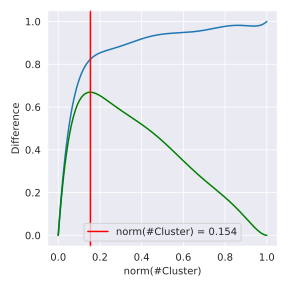
\includegraphics[width=\textwidth]{PCA/Cluster_Knee_Segment_4.pdf}
    \end{subfigure}
    \hfill
    \begin{subfigure}[b]{0.475\textwidth}
        \caption[Kneedle Knee]{\textbf{Kneedle Knee}}
        \label{subfig:PCA_Cluster_Knee_Elbow_4}            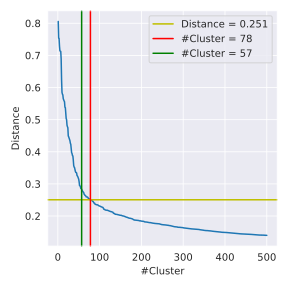
\includegraphics[width=\textwidth]{PCA/Cluster_Elbow_Knee_Segment_4.pdf}
    \end{subfigure}
    \vskip\baselineskip
    \begin{subfigure}[b]{0.475\textwidth}
        \caption[Cluster Distribution]{\textbf{Cluster Distribution}}
        \label{subfig:PCA_Cluster_Knee_Distributione_4}            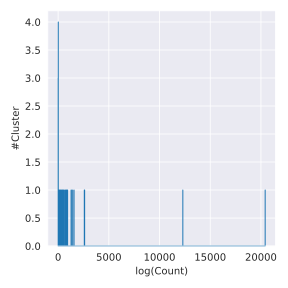
\includegraphics[width=\textwidth]{PCA/Cluster_Distribution_Segment_4.pdf}
    \end{subfigure}
    \hfill
    \begin{subfigure}[b]{0.475\textwidth}
        \caption[Logarithmic Distribution]{\textbf{Logarithmic Distribution}}
        \label{subfig:PCA_Cluster_Knee_Distribution_log_4}            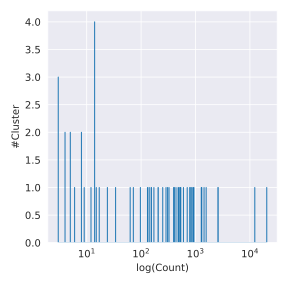
\includegraphics[width=\textwidth]{PCA/Cluster_Distribution_Log_Segment_4.pdf}
    \end{subfigure}
    %\end{adjustbox}
    \caption[Clustering of segment 4 with PK]{\textbf{Clustering of segment 4 with PK.} Segment 4 clustering, using the combination of \texttt{PCA} and the Kneedle Algorithm (PK) results in the given figure. The green curve in the top left sub figure describes the change of the distance in the single linkage tree with increasing normalized cluster number and, therefore, the location of the knee, at the maximum, highlighted by the red line. The blue line is the inverse polynomial representation of the blue line in top right sub figure. The top right sub figure shows the absolute relation of the distance in the single linkage tree to the total number of clusters as the blue line. The red line, indicates the number of raw clusters, by the \texttt{DBSCAN} part of the hybrid \texttt{HDBSCAN} clustering and the final cluster number in green. The yellow line describes the threshold, extracted from the knee and, therefore, the $\varepsilon$ value used to perform the hybrid clustering. The normalized cluster number in the red line in the top left sub figure is equivalent to the raw cluster number in the top right sub figure. The bottom sub figures give information about the distribution of the clusters sizes, by plotting the number of clusters containing a given counted number of sequences in continuous and logarithmic scale.}
    \label{fig:PCA_Cluster_Knee_4}
\end{figure}

A big difference in the cluster size distribution stand out, when comparing the method with \texttt{PCA} (PK) to the ones with \texttt{UMAP} (UK and UD). Only the method using \texttt{PCA} and the Kneedle Algorithm created clusters with more than 10000 vectors (\autoref{subfig:PCA_Cluster_Knee_Distributione_4}). The different cluster sizes using \texttt{UMAP} are spreaded more equally with no cluster of 3000 vectors or more (\autoref{subfig:UMAP_Cluster_DBCV_Distribution_4} and \autoref{subfig:UMAP_Cluster_Knee_Distributione_4}). Since the \texttt{UMAP} methods also use prior \texttt{PCA} reduction, the major difference is the additional use of \texttt{UMAP} (\autoref{sec:Dimension_Reduction}). Therefore, the difference in cluster size distribution was most likely caused by \texttt{UMAP}. \texttt{UMAP} not only reduces the dimension of the data but also changes the position of the vectors in the embedded dimension according to the used settings. The \texttt{n\_neighbors=100} setting seems to be most likely the cause of a change of this magnitude. By increasing the number of neighbors the vectors were more crowded in groups to support the bigger picture of the data and, therefore, seemed to build more crowded clusters of equal sizes. 

\vspace{1em}

With the distribution of segment 4 sequences in the data in \autoref{subfig:Frequency_4} in mind, it was expected that a distribution of cluster sizes in segment 4 clustering would in fact approximate the distribution of the sequences in the former one. Therefore, a clustering with \texttt{PCA} in combination with Kneedle Algorithm exploration seemed to give the expected results and appears again as the best method for \gls{IAV} clustering. Taking also the relation of the cluster number and the distance into consideration \autoref{subfig:PCA_Cluster_Knee_Elbow_4} indicated continuous merging of clusters with decreasing cluster number in the linkage tree and easily distinguishable knee point. The behavior is not present in \autoref{subfig:UMAP_Cluster_Knee_Elbow_4} and \autoref{subfig:UMAP_Cluster_DBCV_Elbow_4} in a similar degree.  

% Also the distribution of cluster sizes seems to be more balanced e.~g.~, segment 4 (\autoref{subfig:UMAP_Cluster_Knee_Distributione_4} and \autoref{subfig:UMAP_Cluster_Knee_Distribution_log_4}) than in the \texttt{PCA} approach (\autoref{subfig:PCA_Cluster_Knee_Distributione_4} and \autoref{subfig:PCA_Cluster_Knee_Distribution_log_4}) which could also contribute to the hybrid clustering by \texttt{DBSCAN} alone. With a more distributed number of sequences in the clusters, less very small and very big clusters exist and overall more points are collected in small groups which decreases the chance for single points unaffected by the $\varepsilon$ threshold. 

\vspace{1em}

The results of the method using \texttt{PCA} in combination with the Kneedle Algorithm (PK) were visualized by the cluster tree \autoref{fig:PCA_Clusteree_Knee_4}. Labeling of the tree was performed based on the \gls{HA} antibody subtype as shown in \autoref{subfig:Frequency_4}. Therefore, clusters only containing sequences of a given subtype are labeled as such. If a cluster only contained sequences of one subtype, plus some not classified sequences, the not classified sequences were declared as the subtype too. That way, a clear presentation of the subtype distribution by labeling was possible, since the not classified sequences were very likely to actually belong to an existing subtype when clustered that way. If they actually did not belong to a existing subtype, a cluster only containing these not classified sequences would most likely have occurred, which is not the case. Furthermore, the chance to eventually break the classification of subtypes by declaring not classified sequences to a existing subtype is not given. The clusters are not based on subtypes in any way and the visualization is only for guidance and not possible for any segments other than 4 and 6 anyway. Also, without this assignment of the not classified sequences, no presentation would be possible since they are distributed over mostly all clusters.

\vspace{1em}

If a cluster contains sequences of more than one subtype plus some not classified sequences, no labeling was performed, since the cluster was not homogeneous for one subtype and a declaration of the unclassified was not possible. In the following the term vector is mostly replaced by sequence to aid the discussion in terms of tree placement and subtype relation. Since the vectors represent the sequences, the terms are linked to each other and used as synonyms. %Exceptions are alignments that did not involve the vector representations, only the sequences. 

\begin{table}[!hbt]
    \centering
    \caption[Unclassified sequences in segment 4 cluster 29 with PK]{\textbf{Unclassified sequences in segment 4 cluster 29 with PK.} The \glspl{MSA} mean distance of the given sequences in comparison to a sample of H9 sequences of the same cluster and a sample of unclassified sequences present in other clusters. Only the first 20 columns are presented here, the full table can be found in the projects GitHub Repository\footnotemark.}
    \label{tab:PCA_Error_4_29}
    \pgfplotstabletypeset[
        every head row/.style={
            before row={
                \toprule
            },
            after row={
                \midrule
            },
        },
        every last row/.style={
            after row={
                ... & ... & ... \\
                \bottomrule
            },
        },
        begin table=\begin{tabular*}{0.75\textwidth},
        end table=\end{tabular*},
        columns={0,1,2},
        columns/0/.style={string type,multicolumn names=l,column name=\textbf{Accession}, column type=@{\extracolsep{\fill}\hspace{6pt}}l},
        columns/1/.style={multicolumn names=l,column name=\textbf{H9}, column type=l},
        columns/2/.style={multicolumn names=l,column name=\textbf{unclassified}, column type=l},
    ]
    {PCA/error_segment_4_cluster_29_difference_head.csv}
\end{table}

The prime example of the not classified sequence annotation is the yellow labeled cluster 29 of subtype H9 (\autoref{fig:PCA_Clusteree_Knee_4} \textbf{\textsf{A}}). While the vectors of all sequences of subtype H9 are accumulated in this single cluster, the cluster size of 1569 is bigger than the number of H9 sequences in \autoref{subfig:Frequency_4} with 1454. This is justified by the presence of 115 not classified sequences in the cluster which are declared as H9, since only H9 and unclassified sequences are present in the cluster. The declaration of the unclassified sequences to be the H9 sequences is supported by the very small evolutionary distance values for the unclassified sequences in comparison to a sample of H9 sequences from the same cluster (\autoref{tab:PCA_Error_4_29}). The sequences were also compared to unclassified sequences from other clusters to prove the smaller evolutionary distance to H9 sequences. This comparison was performed to prove that, even when only used for visualization reasons, the annotation of not classified sequences in that way is most likely true.

\vspace{1em}

The number of clusters for a given subtype of \gls{HA} antibody seems to correspond roughly to the overview of sequences in \autoref{subfig:Frequency_4}. Clusters of very low represented subtypes, like H15, contain mostly all the subtypes sequences, while the high represented subtypes sequences, like H1 and H3, are spreaded over more clusters.

\begin{figure}[!hbt]
    \centering
    \footnotesize
    \begin{tikzpicture}
        \node[anchor=south west,inner sep=0] (image) at (0,0) {\includegraphics[width=\textwidth]{PCA/Clustertree_Segment_4_H_Knee.pdf}};
        \begin{scope}[x={(image.south east)},y={(image.north west)}]
            %\draw[help lines,xstep=.1,ystep=.1] (0,0) grid (1,1);
            \node at (0.16,0.18) [arrowstyle=1.0cm, arrowfillR, anchor=east, rotate=45] {\textbf{\textsf{A}}};
            \node at (0.5,0.08) [arrowstyle=1.0cm, arrowfillR, anchor=east, rotate=45] {\textbf{\textsf{B}}};
            \node at (0.89,0.62) [arrowstyle=1.0cm, arrowfillR, anchor=east, rotate=180] {\rotatebox{180}{\textbf{\textsf{C}}}};
            \node at (0.7,0.9) [arrowstyle=1.0cm, arrowfillR, anchor=east, rotate=180] {\rotatebox{180}{\textbf{\textsf{D}}}};
        \end{scope}
    \end{tikzpicture}

    \caption[Clustering tree of segment 4 with PK]{\textbf{Clustering tree of segment 4 with PK.} The cluster tree of segment 4 clustering, using the combination of \texttt{PCA} and the Kneedle Algorithm (PK) (\autoref{fig:PCA_Cluster_Knee_4}). The labeling of the clusters in the tree is based on the subtype of the contained sequences. Unclassified sequences of a cluster are reclassified as a given subtype if sequences of only this subtype are present in the cluster in addition to the unclassified ones. Unlabeled clusters contain sequences from at least two subtypes and zero or more unclassified sequences. Two clusters are mixed since containing sequences of more than one subtype (\autoref{tab:Cluster_Knee}). These non homogeneous clusters are marked by \textbf{\textsf{B}} and \textbf{\textsf{C}}. The cluster 29 marked by \textbf{\textsf{A}} is an example for an cluster consisting of all sequences from a given subtype. The misplaced cluster from subtype H3 is marked by \textbf{\textsf{D}}. Dotted lines in the tree indicate the same host.}
    \label{fig:PCA_Clusteree_Knee_4}
\end{figure}

Striking anomalies divergent from the expected nearly uniform allocation of the subtypes in \autoref{fig:PCA_Cluster_Knee_4} are noted by \textbf{\textsf{B}}, \textbf{\textsf{C}} and \textbf{\textsf{D}} and are discussed in the following. For final acceptance of the method PK as the prime \gls{IAV} clustering method proposed in this project, the cluster tree was compared to a similar one created on the results from method UK (\autoref{fig:UMAP_Clusteree_Knee_4}. While the labeling of the cluster tree of method PK resemble the subtype classification of \gls{IAV} very closely, no recognizable subtype separation is present in the cluster tree of UK. 
\footnotetext{\url{https://github.com/ahenoch/Masterthesis.git}}

\section{Database Annotation Errors} \label{sec:Clustering_Anomalies}

To evaluate the anomalies in \autoref{fig:PCA_Cluster_Knee_4} \textbf{\textsf{B}} and \textbf{\textsf{C}}, an evolutionary distance was calculated by \gls{MSA} for every eventually misplaced sequence (\autoref{sec:MAFFT}). Therefore, the eventually misplaced sequence was compared to ten other sequences. A sample of five sequences from the same cluster related to the dominant subtype of the cluster, and a sample of five sequences with subtype equal to the misplaced sequence but from other clusters. The mean of distances was then calculated for both cases to rate the assignment and reveal possible misannotations in the \gls{IRD}. 

\begin{table}[!hbt]
    \centering
    \caption[Anomalies in segment 4 cluster 2 with PK]{\textbf{Anomalies in segment 4 cluster 2 with PK.} The \glspl{MSA} mean distance of the given sequences in comparison to a sample of H1 sequences of the same cluster and a sample of H10 sequences present in other clusters.}
    \label{tab:PCA_Error_4_2}
    \pgfplotstabletypeset[
        every head row/.style={
            before row={
                \toprule
            },
            after row={
                \midrule
            },
        },
        every last row/.style={
            after row={
                %... & ... & ... & ... & ... & ... & ... & ...\\
                \bottomrule
            },
        },
        begin table=\begin{tabular*}{0.75\textwidth},
        end table=\end{tabular*},
        columns={0,1,2},
        columns/0/.style={string type,multicolumn names=l,column name=\textbf{Accession}, column type=@{\extracolsep{\fill}\hspace{6pt}}l},
        columns/1/.style={multicolumn names=l,column name=\textbf{H1}, column type=l},
        columns/2/.style={multicolumn names=l,column name=\textbf{H10}, column type=l},
    ]
    {PCA/error_segment_4_cluster_2_difference_head.csv}
\end{table}

In case of \autoref{fig:PCA_Cluster_Knee_4} \textbf{\textsf{C}}, a single sequence with subtype H10 was classified as belonging to cluster 2 which other than that completely consists of H1 and unclassified sequences. By investigation on this possible misplacement, comparison with \gls{MSA} was used. The results for this comparison in \autoref{tab:PCA_Error_4_2} points to the fact, that the as H10 annotated sequence with accession MK237334 is related to subtype H1. The mean of evolutionary distance based on \glspl{MSA} with the sequence and a sample of cluster 0 H1 sequences was very low. Considering the large size of cluster 0 a higher difference was expected, pointing in direction of many very similar sequences in the cluster. Nevertheless, the evolutionary distance of the sequence in comparison to a sample of random H10 sequences was much higher (\autoref{tab:PCA_Error_4_2}). %Even when considering the random sampling of the H10 sequences and the possibility of higher differences of the sequences by origination from different clusters, a misannotation is still more likely. 
Furthermore, only this sole sequence, annotated as subtype H10, was present in a cluster of over 900 sequences of H1 with a very low evolutionary distance to a sequence sample of the cluster, rendering the error most likely as a misannotation.

\begin{table}[!hbt]
    \centering
    \caption[Anomalies in segment 4 cluster 48 with PK]{\textbf{Anomalies in segment 4 cluster 48 with PK.} The \glspl{MSA} mean distance of the given sequences in comparison to a sample of H16 sequences of the same cluster and a sample of H13 sequences present in another cluster. Only the first 20 columns are presented here, the full table can be found in the projects GitHub Repository\footnotemark.}
    \label{tab:PCA_Error_4_48}
    \pgfplotstabletypeset[
        every head row/.style={
            before row={
                \toprule
            },
            after row={
                \midrule
            },
        },
        every last row/.style={
            after row={
                ... & ... & ...\\
                \bottomrule
            },
        },
        begin table=\begin{tabular*}{0.75\textwidth},
        end table=\end{tabular*},
        columns={0,1,2},
        columns/0/.style={string type,multicolumn names=l,column name=\textbf{Accession}, column type=@{\extracolsep{\fill}\hspace{6pt}}l},
        columns/1/.style={multicolumn names=l,column name=\textbf{H16}, column type=l},
        columns/2/.style={multicolumn names=l,column name=\textbf{H13}, column type=l},
    ]
    {PCA/error_segment_4_cluster_48_difference_head.csv}
\end{table}

\footnotetext{\url{https://github.com/ahenoch/Masterthesis.git}}
When comparing the distances for the same calculation performed on \autoref{fig:PCA_Cluster_Knee_4} \textbf{\textsf{C}} in \autoref{tab:PCA_Error_4_48}, no decision for misannotation can be made. The dominant subtype in the cluster 48 is H16 but the sequences of subtype H13 that seem to be misplaced in the cluster have a smaller distance to the sample of sequences from subtype H13. The difference in distance to sample sequences of H13 as well as to sequences of H16 gave indeed no clear finding. Both results are quite similar and the misclustered sequences seem to share much sequence similarity with both subtypes. Maybe the misclustered sequences in cluster 48 point to a more complex classification. Cluster 48 remained a mixed cluster with many sequences from subtype H13 and H16 and, thus, was treated as clustering error. Therefore, subtype H13 and H16 are the focus of investigations of the clustering behavior in the following sections to reveal possible subdivisions responsible for the clustering error.

\begin{figure}[!hbt]
    \centering
    \includegraphics[width=\textwidth]{PCA/Guidetree_segment_4_H_Centroid.pdf}
    \caption[Centroid guidetree of segment 4 with PK]{\textbf{Centroid guidetree of segment 4 with PK.} The guide tree was created by building a \gls{MSA} on the centroid sequences of clusters resulting from the \texttt{PCA} and Kneedle Algorithm (PK) pipeline. The coloring of the tree is based on the related subtype of the centroid sequence used for the \gls{MSA}.}
    \label{fig:PCA_Guidetree_Centroid_4}
\end{figure}

The last error involved cluster 4, that is homogeneous for subtype H3 but is split off the other H3 clusters by nearly all the non H3 clusters \autoref{fig:PCA_Cluster_Knee_4} \textbf{\textsf{D}}. By evaluation of the clusters relation with a \gls{MSA} created guide tree generated from the centroid vectors sequences, the error persists (\autoref{fig:PCA_Guidetree_Centroid_4}). Every of the 55 clusters have a sequence that should best represent the whole cluster, the centroid sequence, calculated as described in \autoref{sec:MAFFT}. When using the guide tree as comparison, the uniform color distribution stood out. Even the centroid of the mentioned cluster 4 is arranged in a line with all the centroids of clusters homogeneous for subtype H3. This subset of centroid sequences used for the guide tree might be to small for a sure proof, but still the centroid sequences should be the most meaningful ones representing the whole cluster and point to a clear subtype separation. Therefore cluster 4 and 48 (\autoref{fig:PCA_Cluster_Knee_4} \textbf{\textsf{C}} and \textbf{\textsf{D}}) remained as identified clustering mistakes and are further examined in the following.

%Übergang zu cluster Comparison durch Centroid Alignment Tree -> H13/H16 Clustertree, Alignmenttree Vergleich -> Cluster H13/H16 Comparison
%fehler im clustering oder fehler in der DAtenbank

\section{K-mer Representation} \label{sec:K_mer_Representation}

\blindtext

% \begin{figure}[!hbt]
%     \includegraphics[width=\dimexpr\textwidth-2\fboxsep-2\fboxrule,fbox]{PCA/Clustertree_Segment_4_H_Knee_Zoom.pdf}
%     \caption[H13/H16 Simple Clustering Example with \Acrshort{PCA}]{\textbf{H13/H16 Simple Clustering Example with \Acrshort{PCA}.} .}
%     \label{fig:PCA_Clusteree_Knee_Zoom}
% \end{figure}

% \begin{figure}[!hbt]
%     \includegraphics[width=\dimexpr\textwidth-2\fboxsep-2\fboxrule,fbox]{UMAP/Clustertree_Segment_4_H_Knee_Zoom.pdf}
%     \caption[H13/H16 Simple Clustering Example with \Acrshort{UMAP}]{\textbf{H13/H16 Simple Clustering Example with \Acrshort{UMAP}.} .}
%     \label{fig:UMAP_Clusteree_Knee_Zoom}
% \end{figure}

% \begin{figure}[!hbt]
%     \includegraphics[width=\dimexpr\textwidth-2\fboxsep-2\fboxrule,fbox]{UMAP/Guidetree_Segment_4_H_Focus.pdf}
%     \caption[H13/H16 Simple Clustering Example with \Acrshort{MSA}]{\textbf{H13/H16 Simple Clustering Example with \Acrshort{MSA}.} .}
%     \label{fig:Guidetree_Focus}
% \end{figure}

\begin{figure}[!hbt]
    \centering
    \includegraphics[width=\dimexpr\textwidth-2\fboxsep-2\fboxrule,fbox]{UMAP/Precalculated_Segment_4_H_Cosine.pdf}
    \caption[H13/H16 Precalculated \Acrshort{UPGMA} Tree (cosine)]{\textbf{H13/H16 Precalculated \Acrshort{UPGMA} Tree (cosine).} .}
    \label{fig:Precalculated_Cosine}
\end{figure}

\begin{figure}[!hbt]
    \centering
    \includegraphics[width=\dimexpr\textwidth-2\fboxsep-2\fboxrule,fbox]{UMAP/Precalculated_Segment_4_H_Euclidean.pdf}
    \caption[H13/H16 Precalculated \Acrshort{UPGMA} Tree (euclidean)]{\textbf{H13/H16 Precalculated \Acrshort{UPGMA} Tree (euclidean).} .}
    \label{fig:Precalculated_Euclid}
\end{figure}

\section{The optimal Clustering Method} \label{sec:Comparison_Clustering}

\blindtext

\begin{figure}[!hbt]
    \centering
    \includegraphics[width=\textwidth]{PCA/Clustertree_Segment_4_H_Simple.pdf}
    \caption[H13/H16 Simple Clustering Example (\Acrshort{PCA})]{\textbf{H13/H16 Simple Clustering Example (\Acrshort{PCA}).} .}
    \label{fig:Simple_Clustertree_PCA}
\end{figure}

\begin{figure}[!hbt]
    \centering
    \includegraphics[width=\textwidth]{UMAP/Clustertree_Segment_4_H_Simple.pdf}
    \caption[H13/H16 Simple Clustering Example (\Acrshort{UMAP})]{\textbf{H13/H16 Simple Clustering Example (\Acrshort{UMAP}).} .}
    \label{fig:Simple_Clustertree_UMAP}
\end{figure}

\begin{figure}[!hbt]
    \centering
    \includegraphics[width=\textwidth]{PCA/Clustertree_Segment_4_H_Focus.pdf}
    \caption[H13/H16 Simple Clustering Example with Guidetree]{\textbf{H13/H16 Simple Clustering Example with Guidetree.} .}
    \label{fig:Simple_Clustertree_MSA}
\end{figure}

\begin{figure}[!hbt]
    \centering
    \includegraphics[width=\textwidth]{PCA/Clustertree_Segment_4_H_Cosine.pdf}
    \caption[H13/H16 Simple Clustering Example with Precalculated (cosine)]{\textbf{H13/H16 Simple Clustering Example with Precalculated (cosine).} .}
    \label{fig:Simple_Clustertree_Cosine}
\end{figure}

\begin{figure}[!hbt]
    \centering
    \includegraphics[width=\textwidth]{PCA/Clustertree_Segment_4_H_Euclidean.pdf}
    \caption[H13/H16 Simple Clustering Example with Precalculated (euclidean)]{\textbf{H13/H16 Simple Clustering Example with Precalculated (euclidean).} .}
    \label{fig:Simple_Clustertree_Euclid}
\end{figure}

\section{The Differences in Dimension Reduction} \label{sec:Dimension_Reduction}

\blindtext

\begin{figure}[!hbt]
    \centering
    \includegraphics[width=\textwidth]{PCA/Difference_Segment_4_H_PCA.pdf}
    \caption[H13/H16 Component Reduction Example (\Acrshort{PCA})]{\textbf{H13/H16 Component Reduction Example (\Acrshort{PCA}).} .}
    \label{fig:Reduction_Example_PCA}
\end{figure}

\begin{figure}[!hbt]
    \centering
    \includegraphics[width=\textwidth]{UMAP/Difference_Segment_4_H_UMAP_Neighbors_10.pdf}
    \caption[H13/H16 Component Reduction Example (\Acrshort{UMAP}, n = 10)]{\textbf{H13/H16 Component Reduction Example (\Acrshort{UMAP}, n = 10).} .}
    \label{fig:Reduction_Example_UMAP_10}
\end{figure}

\begin{figure}[!hbt]
    \centering
    \includegraphics[width=\textwidth]{UMAP/Difference_Segment_4_H_UMAP_Neighbors_50.pdf}
    \caption[H13/H16 Component Reduction Example (\Acrshort{UMAP}, n = 50)]{\textbf{H13/H16 Component Reduction Example (\Acrshort{UMAP}, n = 50).} .}
    \label{fig:Reduction_Example_UMAP_50}
\end{figure}

\begin{figure}[!hbt]
    \centering
    \includegraphics[width=\textwidth]{UMAP/Difference_Segment_4_H_UMAP_Neighbors_100.pdf}
    \caption[H13/H16 Component Reduction Example (\Acrshort{UMAP}, n = 100)]{\textbf{H13/H16 Component Reduction Example (\Acrshort{UMAP}, n = 100).} .}
    \label{fig:Reduction_Example_UMAP_100}
\end{figure}

\begin{figure}[!hbt]
    \centering
    \includegraphics[width=\textwidth]{UMAP/Difference_Segment_4_H_UMAP_Neighbors_200.pdf}
    \caption[H13/H16 Component Reduction Example (\Acrshort{UMAP}, n = 200)]{\textbf{H13/H16 Component Reduction Example (\Acrshort{UMAP}, n = 200).} .}   \label{fig:Reduction_Example_UMAP_200}
\end{figure}

%wichtig erkläre warum dimension reuction mit neigbors 100 und dann feines clustering sinn macht -> HDBSCAN in methoden

\section{A new classification} \label{sec:Serotype_Classification}

\begin{figure}[!hbt]
    \centering
    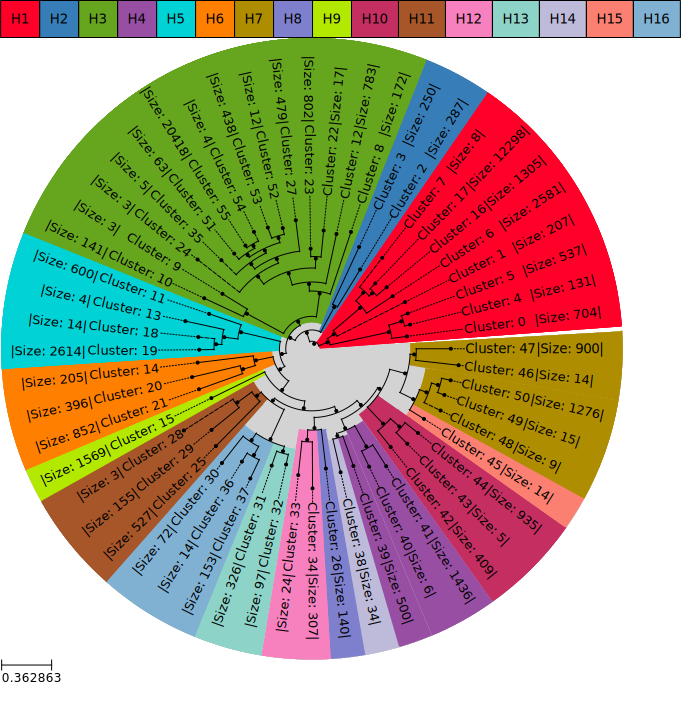
\includegraphics[width=\textwidth]{Results/Clustertree_Segment_4.pdf}
    \caption[Clustering tree of segment 4]{\textbf{Clustering tree of segment 4.} The clustering tree of segment 4 clustering, using the combination of \texttt{PCA} and the Kneedle Algorithm (PK) with a reduction to 50 instead of 30 dimensions (\autoref{fig:PCA_Cluster_Knee_4}). The labeling of the clusters in the tree is based on the subtype of the contained sequences. Unclassified sequences of a cluster are reclassified as a given subtype if sequences of only this subtype are present in the cluster in addition to the unclassified ones. Unlabeled clusters contain sequences from at least two subtypes and zero or more unclassified sequences. Dotted lines in the tree indicate the same host.}
    \label{fig:Result_Clustertree_Segment_4}
\end{figure}

Reannotation of the most likely false annotated sequence in \autoref{fig:PCA_Clusteree_Knee_4} \textbf{\textsf{C}} as well as increasing of the components in \texttt{PCA} successfully raised the accuracy of the pipeline. Thus, the clustering was performed according to the PK method, that proved to give the most stable results, with 50 components reduction instead of 30. Clustering errors found in the previous section were resolved successfully as H13 and H16 are now completely divided, with the mentioned small but still present difference between these subtypes. Also, all clusters of H3 are now present in direct connection to each other and no cluster not homogeneous for one subtype exist anymore. Comparison of the associated clustering information graphics in \autoref{fig:Result_Cluster_Knee_4} to the previous ones in \autoref{sec:Clustering} also indicate a small improvement in stability of the Kneedle Algorithm $\varepsilon$ exploration. Little changes in the distribution of the clustersizes are also noticeable, as a cluster now exist, containing 20000 of the H3 sequences pointing in direction of a merge of two big clusters by the availability of a higher amount of information.  

\vspace{1em}
%neue classification vorschlagen blablabla
% vielleicht bisschen evolution black sea gull etc

Resulting from this improved clustering of segment 4 a new classification involving 57 clusters instead of 18 subtypes is proposed (\autoref{fig:Result_Clustertree_Segment_4}). The big differences in the cluster sizes related to H1 and H3 indicate a high amount of more similar sequences. This can be caused by the higher abundance of more present-day sequences and continued evolution, thus, higher differences in comparison to less sequenced strains of the past decades. Less present mutations lowering the infectiousness and therefore, not established in a higher amount of strains or sequencing errors that produced undesired niches are also possible. These possible error sources have to be examined in the next steps following this project.

\vspace{1em}

By pairwise comparison of random 10 sequence samples of these clusters the similarity inside these clusters is described in \autoref{fig:Proof_Clustertree_Segment_4}. To avoid creating a bias, the result for accidental comparisons of sequences with the same accession are ignored and not considered in calculations of respective mean values. Samples of 10 sequences were used due to the high amount of computational power that is necessary for this calculation. For segment 4 calculation involves $10^2$ pairwise alignments, for every of the 57 clusters to each other. Making $57^2\cdot 10^2$ calculations.

\begin{figure}[!hbt]
    \centering
    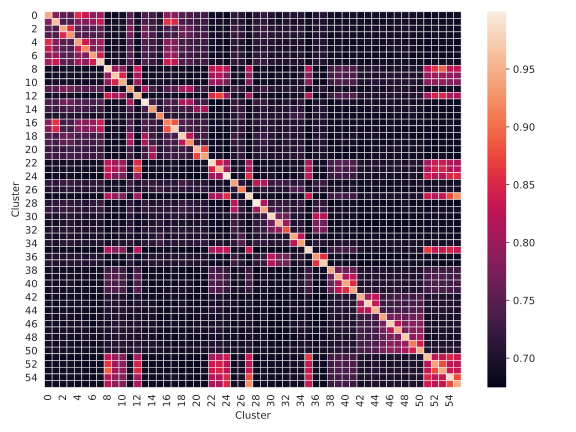
\includegraphics[width=\textwidth]{Results/Cluster_Difference_Segment_4.pdf}
    \caption[Similarity matrix of segment 4 clusters]{\textbf{Similarity matrix of segment 4 clusters.}. Random samples of up to 10 sequences of every cluster in \autoref{fig:Result_Clustertree_Segment_4} were compared by pairwise alignments with the samples of all other clusters. Less than 10 sequences were only used in clusters containing less than 10 sequences. The percentage of similarity was calculated for very alignment making a matrix of up to $10\times10$ holding the similarity values of the samples comparisons. The mean of the matrix was then calculated and written as the given cluster interactions mean similarity. This was repeated for every possible cluster interaction resulting in the presented figure. Interactions of the same clusters were reduced to only different sequences, results of alignments with sequences having the same accession were removed, thereby, preventing bias creation. The mean of these up to 100 comparisons for every cluster interaction are colored according to their similarity from 1.0 or 100\% similarity in red to 0.0 or 0\% similarity in blue.}
    \label{fig:Proof_Clustertree_Segment_4}
\end{figure}

\vspace{1em}

All clusters in \autoref{fig:Proof_Clustertree_Segment_4} have the highest similarities with themselves and mostly high similarities with clusters of the same subtype. For instance cluster 0, share some degree of sequence identity with other clusters stemming from the same subtype H1, as shown in \autoref{fig:Proof_Clustertree_Segment_4}. However, the highest similarity of around 90\% is only shared with other sequences of the cluster itself, which makes this cluster very self contained. 

\vspace{1em}

Exceptions are the subtype H7 and H15 clusters 45 to 50, as well as subtype H4 and H14 clusters 35 to 38, that share a high degree of similarity despite of the subtype difference \autoref{fig:Proof_Clustertree_Segment_4}. In the clustering tree no clear separation was performed involving these subtypes as the clusters of H7 merge with H15 in a higher tree nodes, although other clusters of H7 are still available (\autoref{fig:Result_Clustertree_Segment_4}). Similar behavior can be observed for H4 with H14. These same merges were also present in the previous clustering with reduction to 30 dimensions (\autoref{fig:PCA_Clusteree_Knee_4}). Due to the high similarities inside these two groups of clusters, a relation neglected by the current subtype classification could be possible. The almost uniform H7 subtree of clusters 45, 46, 48, 49, and 50 is, therefore, divided by the one and only cluster of subtype H15 cluster 47. When comparing the sequence similarities in \autoref{fig:Proof_Clustertree_Segment_4}, the highest similarity persist inside the clusters themselves, but the cross similarities of cluster 45 and 46 to 47, 48, 49, and 50 are around 65\% without big difference between subtype H7 and H15. Further pointing to more subtle but present differences between and inside of the current subtypes. Aside from that, the amount of information preserved by the \texttt{PCA} can still be to small to fully separate the subtypes H4 and H14 and the subtypes H7 and H15, that possibly involve even more subtle differences than the previously discussed separation of H13 and H16. The inclusion of evolution into the vectors as described in the following could be the necessary step to increase the amount of information without further raising the components by \texttt{PCA} to successfully separate these subtypes. Still, all the clusters are homogeneous for one subtype, only the position in the tree could be inaccurate and, therefore, should be subject of improvements.  

\vspace{1em}

With this pipeline blueprint created by adjusting the clustering for segment 4 in the previous sections, all \gls{IAV} segments could be clustered the same way, since no subtype information is necessary for the clustering. Subtype labeling of the tree was performed as guideline and was the only part involving actual sequence position to subtype evaluation. Thereby, the clustering trees for other segments, except segment 6, are unlabeled. All other clustering trees and similarity matrix graphics, as well as tables containing sequence cluster assignment and the tables containing the values used to create the graphics are presented in the \autoref{chap:Appendix}. Hereby new classifications for all segments based on $k$-mer frequency vectors are proposed, containing 28 clusters for segment 1, 28 for segment 2, 29 for segment 3, the shown 57 for segment 4, 26 for segment 5, 40 for segment 6, 30 for segment 7 and 24 clusters for segment 8 \autoref{tab:Result_Cluster}. 

\vspace{1em}

The clusters of the segments 1 to 3, 5, 7, and 8 share by far more overall similarity, therefore, less clusters were created (\autoref{chap:Appendix}). Still, the similarity inside the clusters themselves is higher than the cross similarity and, thereby, solid clustering by the proposed clustering method was possible despite the overall higher similarity. Higher similarity of the segments not encoding the surface protein is most likely reasoned by the lower evolutionary pressure. The higher pressure of the surface proteins is necessary to ensure infection of the host cells. 

\vspace{1em}

While the clusters of segment 4 seem to be very self contained and give a good representation on possible subdivisions inside the subtypes, the trees based on evolutionary distances increase the subtypes distance even more (\autoref{fig:PCA_Guidetree_Centroid_4} and \autoref{fig:Simple_Clustertree_MSA}). Present day research propose a phylogenic tree of \gls{IAV} that is split in four subtrees \autocite{wei_next-generation_2020}. The subdivisions are mostly present in the clustering tree in \autoref{fig:Result_Clustertree_Segment_4}. Still, there are some difference primarily the higher-ranking structure of the subtypes. In \textcite{wei_next-generation_2020} subtype H3 is contained in a subtree alongside H4 and H14 and H9 in a subtree with H8 and H12. This relations are not present in \autoref{fig:Result_Clustertree_Segment_4}. Though, other subtrees contain subtypes similar to the proposed phylogenic tree in \textcite{wei_next-generation_2020}. Aside from that, the order of the subtrees in \autoref{fig:Result_Clustertree_Segment_4} do not match the one from the pyhlogenic tree.

\begin{figure}[!hbt]
    \centering
    \includegraphics[width=0.5\textwidth]{Graphics/Transition.pdf}
    \caption[7-mer vector calculation involving transitions]{\textbf{7-mer vector calculation involving transitions.} By changing \autoref{fig:k-mer} to include e.~g.~, all transitions possible with one mutation, evolutionary distance can be included in the vectors themselves. Thereby, vectors involving sequences different by a small amount of mutations with higher evolutionary significance move closer to each other. All weightings used here are only exemplary and useful values have to be selected in the future based on novel publications  involving mutation probabilities.}
    \label{fig:trans}
\end{figure}

As already mentioned the proposed method for \gls{IAV} clustering did not acknowledge evolutionary distances. Transitions and transversion for example are handled as nucleotide differences without a higher or lower chance of change. When including mutation chances in the $k$-mer frequency clustering, the relation of whole subtypes subtrees might improve and give a result more similar to the one proposed in \textcite{wei_next-generation_2020}. Because \texttt{HDBCSCAN} only uses existing distance metrics, when not using the precalculated option, which should be avoided at any case, the $k$-mer frequency vectors themselves have to be change in some way. Therefore, \autoref{fig:trans} illustrate a possible option for inclusion of evolution inside $k$-mer frequency vectors, by considering all mutations of a given $k$-mer with low representation value. Vectors containing $k$-mers only apart with single mutations are, thus, closer to each other in the high-dimensional vector space. The magnitude of these values have to be considered wisely and should be subject of future research optimizing the proposed clustering even more. For choice of appropriate values representing the transversions or transitions consideration of PAM or BLOSUM substitution matrices could be beneficial \autocite{mount_comparison_2008}. Since $k$-mers of a sequence are generated by shifting a window of size $k$ by one, all \gls{AA} constellations are automatically included, independent of the $k$ value itself. Thereby, weighting of the mutation possibility could be also implemented by considering the actual $k$-mer with a fixed value e.~g.~ 0.85 and the mutations with fractures of 0.15 given by the priority in the BLOSUM or the PAM matrices. Summing up the values would, thus, still result in one but the weightings are distributed based score of the \gls{AA} change. Expanding the minimal example \autoref{fig:trans} in that way, involving BLOSUM could result in CAA $\rightarrow 0.85$, CAG $\rightarrow \frac{0.15}{(5+1+0)}\cdot 5$, CGA $\rightarrow \frac{0.15}{(5+1+0)}\cdot 1$, and TAA $\rightarrow \frac{0.15}{(5+1+0)}\cdot 0$. The portion of 0.15 is divided by the sum of all considered \glspl{AA} change values and subsequently multiplied by the value of the given one.